\documentclass[12pt,a4paper,titlepage]{report}
% set line spacing to 1.5 and font to Times
\renewcommand{\baselinestretch}{1.5}
\usepackage{times}

\usepackage[
backend=biber,
style=ieee,
citestyle=ieee
]{biblatex}
\addbibresource{../final-report/references.bib}

\usepackage{graphicx}
\usepackage{amssymb}

\usepackage{pdfpages}

\usepackage{indentfirst}

\newcommand{\todo[1]}{\textcolor{red}{#1}}
\let\code\texttt

\begin{document}

\section*{Problem Overview}
	% Explanation of pneumonia
	Pneumonia is an inflammation of the lungs which can be caused by either a fungal, bacterial or viral infection. Of these bacterial or viral infection are the more common cause\todo{source}. According to the \textit{The European Lung white book; Respiratory Health and Disease in Europe} it had a mortality rate in Ireland of 32.96 per 100,000 in 2011\cite{pne-death-rate}, which, when compared to the total death rate in Ireland for 2011 of 6.2 per 1,000, means that pneumonia was responsible for 5.3\% of deaths in Ireland in 2011. \todo{More prevalent in children and elderly}. \par
	% Diagnosis mehtods and use of deep learning in medicine
	There are a number of methods to reliably rule in or out pneumonia when diagnosing a patient, such as the lack of certain symptoms or the presence of rates and bronchial breathing sounds, but chest radiography is generally considered the best method of confirming a pneumonia diagnosis\cite{pne-diagnosis}. There has been a great amount of research into the use of deep learning in medical diagnosis in recent years, in particular for use image-based diagnosis, such as MRI, CAT or X-Rays\cite{pne-ml-in-medicine}. \todo{Examples of ML for diagnosis}. These models are often able to achieve comparable, or sometimes higher, detection rates of these diseases compared to doctors, making them very useful tools. \par
	% Details on dataset
	This example problem aims to demonstrate how a machine learning model could be developed for detecting pneumonia from chest x-rays. It uses chest x-rays from the \textit{Labeled Optical Coherence Tomography (OCT) and Chest X-Ray Images for Classification} dataset\cite{pne-dataset}\footnote{Version 2} produced by Daniel Kermany, Kang Zhang and Michael Goldbaumusing and is used under the Creative Commons \textit{CC BY 4.0} license. This dataset contains 5856 images split into 3 directories; a training directory of 5216 images; a testing directory containing 624 images; and a validation directory containing 16 images. Pneumonia is prevalent in around 75\% of the training presentations, and 50\% of the test presentations. A number of deep learning methods will be explored, but only convolutional neural network (CNNs) models will be used, as almost all real world models for image-based medical diagnosis use CNNs\cite{pne-ml-in-medicine}. \par

\section*{Convolutional Neural Networks}
	% Explanation of CNNs
	Convolutional neural networks (CNNs) are a class of neural networks which use convolutional layers to extract translation invariant \textit{features} from an \textit{feature map}, which can be any matrix $m \in \mathbb{R}^{w \times h \times d}$\cite{cnn-analysis}, such as an image. These features can then be passed as a vector to a neural network and the neural network can then be trained as usual. CNN classification models can generally be broken up into two distinct blocks of layers; a set of layers for feature extraction, and a set of layers for classification. \par
	\begin{figure}[h!]
  		\centering
  		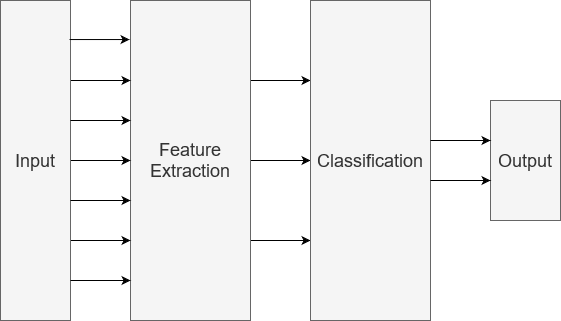
\includegraphics[width=0.7\linewidth]{../final-report/images/cnn_block_diagram.png}
  		\caption{Block diagram of typical CNN}
  		\label{fig:cnn-block}
	\end{figure}
	Despite being shown to be effective at solving machine vision tasks and fully trainable by back-propagation since 1989\cite{cnn-backprop}, it was not until as recently as 2012, when a CNN achieved a top-5 test error rate of 15.3\%, compared to next highest of 26.3\% in the ImageNet challenge\cite{cnn-image-net} that they were considered state-of-the-art. \par
	
	% Explanation of layers and keras implementations
	There are three types of layer typically found in the feature extraction block of a CNN model; Convolutional layers, pooling layers, and normalization layers\cite{cnn-analysis}. Keras\cite{keras} has a number of built in  implementations of these layers to allow their use in models.
	\subsection*{Convolutional Layers}
	Similar to how perceptrons were designed to approximate the neurons in the brain, units in convolutional layers were designed to replicate the cells found in the visual cortex, which have a receptive field, and respond regions of the visual field\cite{cnn-biology}. To do this, convolutional layers use a number, $n$, of filters as their base units, which when convolved with an input feature map produce $n$ output feature maps. The filters, commonly called kernels, are matrices of weights $w \in \mathbb{R}$ of size $k_w \times k_h$ where $k_w, k_h \in \mathbb{N}_{\geq1}$\cite{cnn-analysis}.
%	\begin{figure}[h!]
%  		\centering
%  		\includegraphics[width=0.7\linewidth]{../final-report/images/conv-explain.png}
%  		\caption{Diagram showing convolution of kernel with feature map}
%  		\label{fig:cnn-explain}
%	\end{figure}
	This creates a number of hyperparameters needed to define a convolutional layer;
	\begin{itemize}
	\item $n$, the number of filters,
	\item $(k_w, k_h)$ the shape of the filters, typically square,
	\item the activation function for the layer, which should be non-linear (similar to a normal perceptron layer),
	\item the stride $s \in \mathbb{N}_{\geq1}$, which defines how much to move the kernel by when doing the convolutional,
	\item and the padding, which is used to determine the values convolved with the filter when it overlaps the edges of the image.
	\end{itemize}
	Keras offers a number of implementations of convolutional layers in the \code{keras.layers} module, covering several subtypes of convolutional layer, and with a number of arguments to set the hyperparmeters mentioned above;
	\begin{itemize}
	\item Basic convolution; basic convolutional layers with various shapes of filter, such as 1D, 2D and 3D are offered by \code{Conv1D}, \code{Conv2D} and \code{Conv3D} respectively.
	\item Depthwise separable convolution; when dealing with images with multiple channels, such as an RGB image, the number of multiplications done during convolution can get very large. To reduce the number of multiplications done, depthwise convolution can be done instead, convolving each channel of the image separably, and then the channels can be combined using a $1 \times 1 \times d$ kernel. This produces the same result as a regular convolution, but requires far fewer multiplications, and also fewer parameters\cite{cnn-depth-conv}. This is implemented in the keras layers \code{SeparableConv1D} and \code{SeparableConv2D}.
	\item Depthwise convolution; if only a depthwise convolution is desired, i.e. a convolution on each input channel individually without combining afterwards, then a \code{DepthwiseConv2D} layer can be used.
	\end{itemize}
	
	\subsection*{Pooling Layers}
	Pooling is used to reduce the size of a feature map, while trying to retain the features. This is done by creating a summary of $p \times p$ areas of the image. The summary is created by applying a function to the pooled area, commonly used functions being; max pooling, taking the maximum value in the area; average pooling, taking the mean of an area; $l_2$ pooling, which takes the $l_2$ norm of the pooled area; and stochastic pooling, which selects a value for each area using its activation value to compute a probability.\cite{cnn-analysis}.
	
	\subsection*{Normalization Layers}
	

\section*{Dataset}
	\todo{Images from dataset, Examples of pneumonia vs normal, etc.}

\section*{Explored Solutions}
	While trying to develop a suitable model for this problem, a number of solutions were looked at, each of increasing complexity\todo{maybe change}, but each achieving better results.
	\subsection*{Simple CNN}
	The first solution looked at was a simple convolutional neural network, based on \todo{similar model on kaggle}. This was composed of 3 convolutional layers, with a $3\times3$ kernel size, and rectified linear activation function, each followed by a max-pooling layer, with a $2\times2$ pool size. After these convolutional layers a dense layer of 64 neurons, again using the rectified linear activation function, before a single neuron output layer, using a sigmoid activation function to create a binary classifier. \\
	\todo{Add some images} \\
	\todo{Add training info/accuracy} \\
	\todo{Comments}
	\subsection*{Image Augmentation}
	Image augmentation is the \todo{find word, technique?} of performing transformations on the training images, to try stop the model from learning the  \textit{'noise'} in the dataset, and instead learn the desired features\todo{source}. The hope being that by applying semi-random augmentations to the images before they are shown to the system, undesired information will become more random and the system will learn less about it. The Keras \textit{ImageDataGenerator} has a number of arguments that can be used to apply transformations to images as they are presented, such as:
	\begin{itemize}
		\item Rotations; An integer can be passed to set the limit in degrees for random rotations to apply to the image using the \verb!rotation_range! keyword argument
		\item Shifts; The image can be shifted vertically or horizontally by a random number of pixels using the \verb!width_shift_range! and \verb!height_shift_range! keyword arguments.
		\item Mirroring; The image may 50\% of the time be mirrored around either the vertical or horizontal axis using the \verb!horizontal_flip! and \verb!vertical_flip! keyword arguments.
		\item \todo{maybe add in shear, etc.}
	\end{itemize}
	By using these, the performance of the simple CNN described previously can be marginally \todo{(?)} improved. \\ For this example problem, both vertical and horizontal shifts were applied, as well as mirroring across the vertical axis. These transformations were chosen as x-rays may not be centred, so one should still create a plausible input. Similarly as there is no difference between pneumonia in the left and the right lung, flipping the image vertically should not matter.
	\todo{info about this training}
	\subsection*{Transfer Learning}


\printbibliography

\end{document}